\documentclass[a4paper,12pt]{report}
\usepackage[margin=25mm]{geometry}

\usepackage[default]{lato}

\usepackage[brazil]{babel}
\usepackage[utf8]{inputenc}
\usepackage{hyperref}
\usepackage{eso-pic,graphicx}
\usepackage{array, makecell}
\usepackage{enumerate}
\usepackage{enumitem}
\usepackage{graphicx}			% Inclusão de gráficos
\usepackage{caption}			% conFigurar o caption das Figuras e tabelas % Class memoir Warning: You are using the caption package with the memoir class.
% separação entre colunas de tabelas
\usepackage{placeins}
\usepackage{titlesec}   
\usepackage{subfig}

\usepackage{listings}	
\usepackage{setspace}
% for creating language style
% -------------------------------------------------------
\definecolor{Code}{rgb}{0,0,0}
\definecolor{Decorators}{rgb}{0.5,0.5,0.5}
\definecolor{Numbers}{rgb}{0.5,0,0}
\definecolor{MatchingBrackets}{rgb}{0.25,0.5,0.5}
\definecolor{Keywords}{rgb}{0,0,1}
\definecolor{self}{rgb}{0,0,0}
\definecolor{Strings}{rgb}{0,0.63,0}
\definecolor{Comments}{rgb}{0,0.63,1}
\definecolor{Backquotes}{rgb}{0,0,0}
\definecolor{Classname}{rgb}{0,0,0}
\definecolor{FunctionName}{rgb}{0,0,0}
\definecolor{Operators}{rgb}{0,0,0}
\definecolor{Background}{rgb}{0.98,0.98,0.98}
\lstdefinelanguage{Python}{
	numbers=left,
	numberstyle=\footnotesize,
	numbersep=1em,
	xleftmargin=1em,
	framextopmargin=2em,
	framexbottommargin=2em,
	showspaces=false,
	showtabs=false,
	showstringspaces=false,
	frame=l,
	tabsize=4,
	% Basic
	basicstyle=\ttfamily\small\setstretch{1},
	backgroundcolor=\color{Background},
	% Comments
	commentstyle=\color{Comments}\slshape,
	% Strings
	stringstyle=\color{Strings},
	morecomment=[s][\color{Strings}]{"""}{"""},
	morecomment=[s][\color{Strings}]{'''}{'''},
	% keywords
	morekeywords={import,from,class,def,for,while,if,is,in,elif,else,not,and,or,print,break,continue,return,True,False,None,access,as,,del,except,exec,finally,global,import,lambda,pass,print,raise,try,assert},
	keywordstyle={\color{Keywords}\bfseries},
	% additional keywords
	%morekeywords={[2]@invariant,pylab,numpy,np,scipy},
	keywordstyle={[2]\color{Decorators}\slshape},
	emph={self},
	emphstyle={\color{self}\slshape},
	%
}
% -------------------------------------------------------


\graphicspath{{Figuras/}}
\setlength{\tabcolsep}{0.05cm}
\setlength{\parindent}{0.0cm}
\setlength{\parskip}{0.4cm}  % tente também \onelineskip
%-----------------------------------------------------------------------------------------------
% Define a centralização de coluna com largura {|C{1 cm}|}
\newcolumntype{C}[1]{>{\centering\let\newline\\\arraybackslash\hspace{0pt}}m{#1}}
\newcolumntype{L}[1]{>{\raggedright\let\newline\\\arraybackslash\hspace{0pt}}m{#1}}

% Controle de linhas orfãs e viuvas
\widowpenalty = 10000
\clubpenalty = 10000

\titleformat{\chapter}
{\Large\bfseries} % format
{}                % label
{0pt}             % sep
{\LARGE}           % before-code
% ======================================================================
\makeatletter
\hypersetup{
	%pagebackref=true,
%	pdftitle={\@title}, 
%	pdfauthor={\@author},
%	pdfsubject={\imprimirpreambulo},
	pdfcreator={YuLab tecnologia},
	pdfkeywords={YuLab tecnologia}{Guia Didático Workshop}{Workshop Machine Learning utilizando Python}, 
	colorlinks=true,       		% false: boxed links; true: colored links
	linkcolor=black,          	% color of internal links
	citecolor=black,        		% color of links to bibliography
	filecolor=black,      		% color of file links
	urlcolor=blue,
	bookmarksdepth=4
}
% ---
\newcommand\BackgroundPicture[3]{%
\setlength{\unitlength}{1pt}%
   \put(0,\strip@pt\paperheight){%
      \parbox[t][\paperheight]{\paperwidth}{%
         \vfill
         \centering\includegraphics[width=#2,angle=#3]{#1}
         \vfill
      }
   }
} 
\makeatother
% ======================================================================
% --- Adiciona Timbre --------------------------------------------------
\AddToShipoutPicture{\BackgroundPicture{fundo-de-paginas}{21cm}{0}}
% ----------------------------------------------------------------------

\begin{document}

%%
%% Folha de Rosto
%%
\pagebreak
\thispagestyle{empty}

\begin{center}
  \LARGE{YULAB tecnologia}\\
\end{center}

\begin{center}
	
\includegraphics[keepaspectratio, width=8cm]{BeMaker_Marca_04.pdf}
\end{center}

\vspace{1cm}
\begin{center}
  \Huge{\textbf{Workshop Machine Learning utilizando Python}}\\
  \Large{\textbf{Guia didático}}
\end{center}

\vspace{3cm}
\begin{flushright}
  \begin{minipage}[t]{0.750\textwidth}
Imaginar, desenvolver, construir, aproximar, integrar, amadurecer e evoluir!
Se você teve uma grande ideia, provavelmente passou por este ciclo, é a melhor forma de criar um sucesso. Com essas palavras em mente, construímos a Bemaker! Um makerspace
que nasceu da vontade de impulsionar o movimento \textit{Do It Yourself} (Faça você mesmo) para qualquer esfera da sociedade.
Nossa missão é disponibilizar um espaço com ferramentas para que você construa seus sonhos!
Venha fazer parte deste movimento!
  \end{minipage}
\end{flushright}

\vspace{2cm}
\begin{large}
  \textbf{Autores:}
\end{large}
\begin{itemize} [noitemsep,topsep=0pt]
 \item[--] Adelino Pinheiro Silva (\href{mailto:adelino@yulab.com.br}{adelino@yulab.com.br})
 \item[--] Fabiano Calado (\href{mailto:fabiano@yulab.com.br}{fabiano@yulab.com.br})
 \item[--] Lucas Calado Alves Pereira (\href{mailto:kalado@yulab.com.br}{kalado@yulab.com.br})
 \item[--] Thiago Amaral (\href{mailto:thiago@yulab.com.br}{thiago@yulab.com.br})
\end{itemize}

\vspace{1cm}
\begin{center}

\includegraphics[keepaspectratio, width=2cm]{CC-BY_icon.pdf}
\end{center}

\pagebreak
\thispagestyle{empty}

\chapter{Contextualização}

Este é um guia didático com objetivo de introduzir as técnicas de aprendizado de máquina e aplicá-las na prática. Este material é uma adaptação do guia de Helge Bjorland - \href{https://www.kaggle.com/helgejo/an-interactive-data-science-tutorial}{An Interactive Data Science Tutorial}.

A ferramenta utilizada será o \href{https://pypi.org/project/spyder/}{Spyder} (que pode ser baixado no link) que roda em ambiente \href{https://www.python.org/}{Python}. As demais ferramentas são os pacotes da biblioteca \href{https://www.scipy.org/}{SciPy}. 

O código completo para este workshp pode ser obtido \href{www.cefala.org/~adelino/adelinocpp/YuLab/Workshop/WS_MachineLearning_v2.py}{neste link}.

\section{Ambiente Spyder}

O Spyder é uma interface de desenvolvimento integrada (IDE) para programação em Phyton que agrega algumas funcionalidades como a interpretação interativa.

A tela principal do Spyder pode ser visualizada na Figura~\ref{Fig:Spyder_Tela_01}.

\begin{figure}[h]
	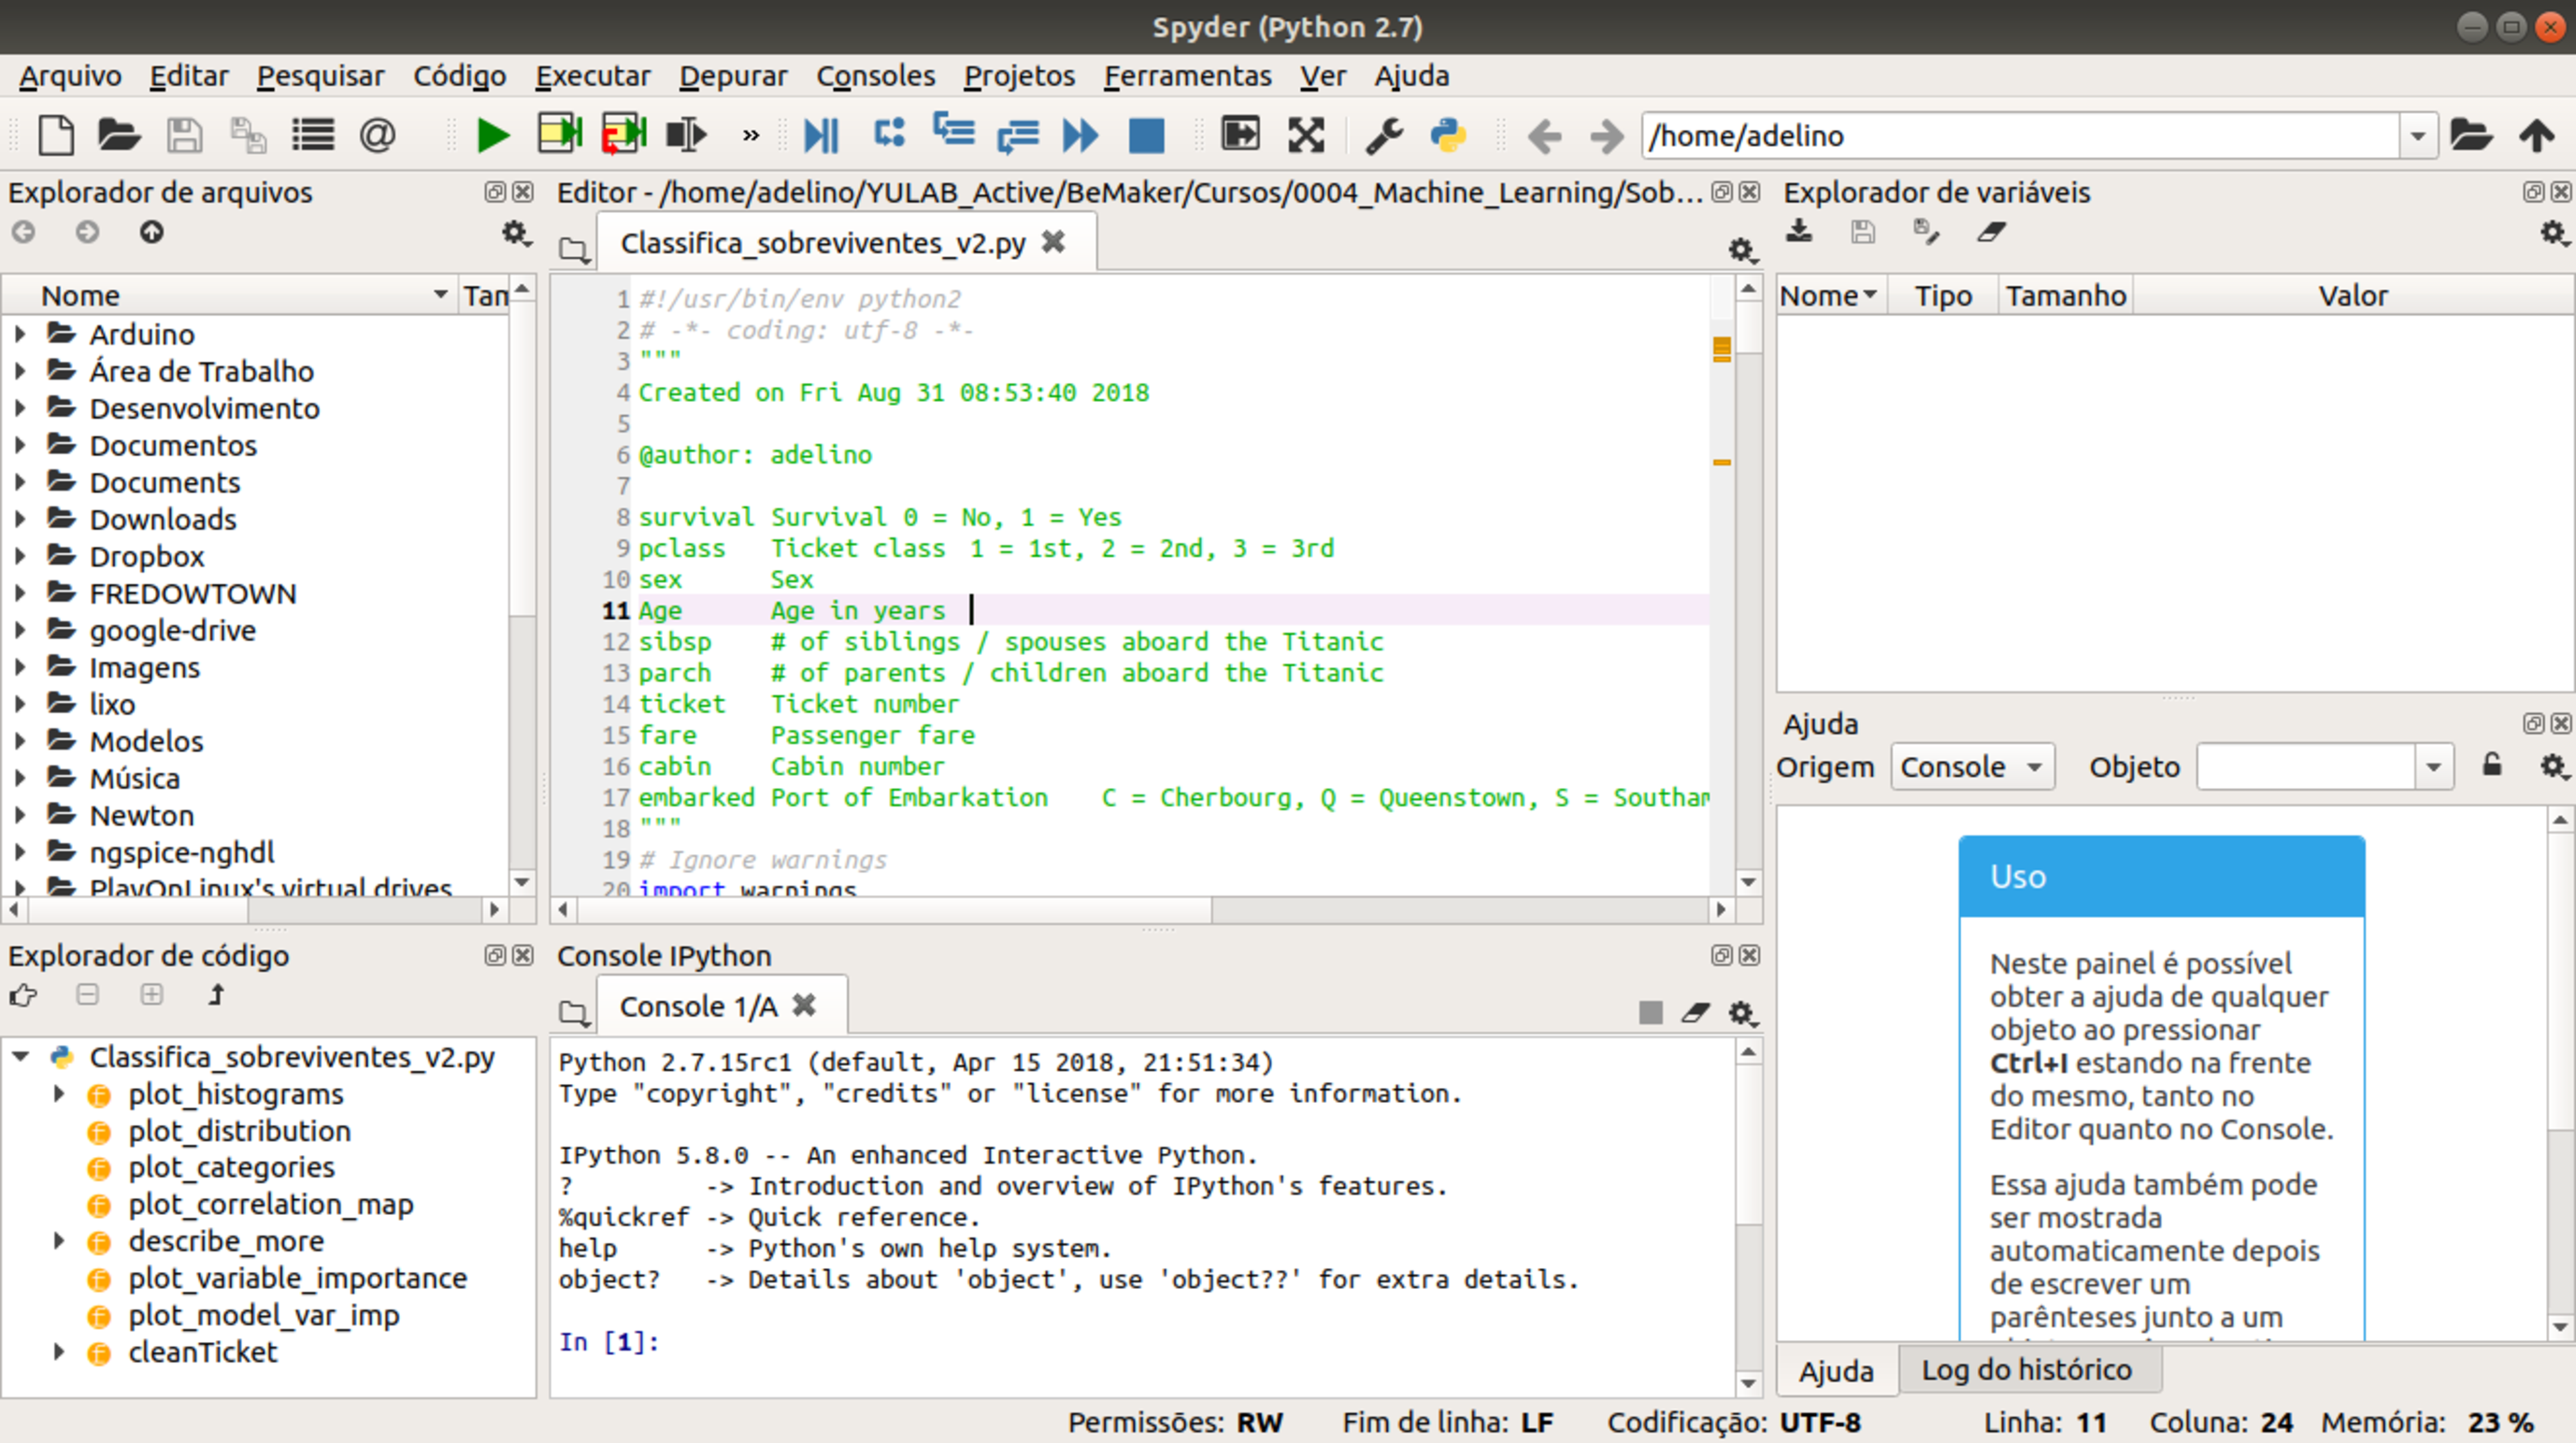
\includegraphics[keepaspectratio, width=\textwidth]{Spyder_tela_01.pdf}
	\caption{Tela de trabalho do Spyder como \textit{layout} do Matlab.}
	\label{Fig:Spyder_Tela_01}
\end{figure}

Na tela do Spyder tem-se várias funcionalidades.  As mais utilizadas são: a janela para o código, que é interpretado de forma interativa pelo Iphyton; a lista de variáveis e o console (ou \textit{prompt}) de comando.

Uma dica importante, para que os gráficos gerados apareçam em uma nova janela, e não no console siga o seguinte menu e altere a variável \texttt{Graphics backend} para \texttt{Automatic}.

Tools $>$ preferences $>$ IPython console $>$ Graphics $>$ Graphics backend $>$ Backend: Automatic

Em seguida reinicie o \textit{kernel} do Iphyton com \texttt{Ctrl+.}.

\chapter{Colocando a mão na massa}

Nesta etapa vamos colocar a mão na massa e programar no ambiente Spyder. O objetivo principal é utilizar as principais ferramentas de aprendizado de máquina sem se aprofundar na teoria.

\section{Compreensão e Visualização dos Dados}



\subsection{Importando as bibliotecas}

O primeiro passo é preparar o ambiente para manipular os dados. O bloco de código abaixo carregas as principais bibliotecas que serão utilizadas no desenvolvimento.\\

\lstinputlisting[language=Python,basicstyle=\footnotesize]{Spyder/1.py}

	
\subsection{Definindo funções auxiliares}

A linguagem Python também permite fazer o encapsulamento de blocos de códigos. O tutorial original não explica o funcionamento das funções. 

Basicamente são funções para visualização de dados.\\

\lstinputlisting[language=Python,basicstyle=\footnotesize]{Spyder/2.py}

\subsection{Carregando dados}

Está é uma etapa importante para qualquer tarefa de aprendizado de máquina. Os dados são toda informação disponível para superar os desafios. 

Basicamente existem dois conjuntos de dados, os de trinamento e os de teste. 

O conjunto de treinamento apresenta dos dados do problema, ou seja, as informações de entrada, e o resultado esperado. Este conjunto permite validar como o aprendizado de máquina esta calibrado. 

Com os dados de teste verifica-se o poder de generalização do aprendizado de máquina.

O bloco de código a seguir é utilizado para carregar e fazer uma visualização prévia nos dados.\\

\lstinputlisting[language=Python,basicstyle=\footnotesize]{Spyder/3.py}

Para se familiarizar com os dados é possível acessar algumas linhas da tabela com o comando \texttt{titanic.head()}.

Basicamente os dados apresentam as seguintes informações:

\begin{enumerate}
	\item \textbf{survival}: Indica de o passageiro foi um sobrevivente ou não, se o valor for 0 é um não sobrevivente e se o valor for 1 é um sobrevivente.
	\item \textbf{pclass}: é a classe que a passagem dá acesso. Neste caso tem-se passagens de 1$^a$, 2$^a$ e 3$^a$ classe.
	\item \textbf{Name}: Nome do passageiro.
	\item \textbf{sex}: sexo do passageiro, e uma variável categórica, sendo \texttt{male} ou \texttt{female}.
	\item \textbf{Age}: idade em anos.
	\item \textbf{sibsp}: número de irmãos ou cônjuges abordo do Titanic.
	\item \textbf{parch}: número de pais ou filhos abordo do Titanic.
	\item \textbf{ticket}: número da passagem.		
	\item \textbf{faer}: valor da tarifa paga pelo passageiro.
	\item \textbf{cabin}: Número da cabine.
	\item \textbf{embarked}: Variável categória que indica o porto em que o passageiro embarcou, sendo \texttt{C} para Cherbourg, \texttt{Q} para Queenstown e \texttt{S} para Southampton.
\end{enumerate}

Uma variável numérica é aquela que apresenta valores inteiros ou números reais, enquanto a variável categórica assume apenas um número limitado, e geralmente fixo, de valores possíveis, como por exemplo o tipo sanguíneo ou o sexo.

\subsection{Visualização de variáveis numéricas}

%\lstinputlisting[language=Python,basicstyle=\footnotesize]{Spyder/5.py}

%\lstinputlisting[language=Python,basicstyle=\footnotesize]{Spyder/6.py}

A sequência de código a seguir permite verificar como as variáveis numéricas se distribuem. \\

\lstinputlisting[language=Python,basicstyle=\footnotesize]{Spyder/4.py}

O desafio desta etapa é verificar as variáveis correlacionadas e entender como elas podem explicar o problema.

\subsubsection{Exercício 1: Investigando as taxas de sobrevivência}

Nesta etapas vamos o primeiro exercício, gerar gráficos que indique os índices de sobrevivência de acordo com as variáveis do problema.

Este é um exemplo de figura que pode ser gerada.

\begin{figure}[h]
	\centering
	
\includegraphics[keepaspectratio, width=0.5\textwidth]{Parch_Survived_v0.pdf}
	\caption{Taxa de sobrevivência de acordo com o numero de pais e filhos a bordo.}
	\label{Fig:Exemplo_01}
\end{figure}

\subsection{Visualização de variáveis categóricas}

As variáveis \texttt{Embarked}, \texttt{Pclass} e \texttt{Sex} são tratadas nos dados como variáveis categóricas. Como os algoritmos recebem variáveis numéricas, faz-se necessário criar variáveis numéricas relacionadas às variáveis categóricas. 

Desta forma, cada variável poderá assumir os valores 0 ou 1 se forem inseridas na em determinada categoria. Por exemplo, para o sexo, cria-se uma variável chamada \texttt{male} e o ``valor'' será codificado como uma variável binária (0 ou 1). \\

\lstinputlisting[language=Python,basicstyle=\footnotesize]{Spyder/8.py}

\section{Preparação dos Dados}

\subsection{Variáveis ausentes}

A maioria dos algoritmos de aprendizado de máquina exige que todas as variáveis tenham valores para usá-lo no treinamento do modelo. O método mais simples é preencher os valores ausentes com a média da variável em todas as observações no conjunto de treinamento.\\

\lstinputlisting[language=Python,basicstyle=\footnotesize]{Spyder/9.py}

\section{Engenharia de Características/Recursos - Criação de novas variáveis}



\subsection{Títulos dos nomes dos passageiros}

Títulos refletem status social. No caso do Titanic. estes títulos podem prever probabilidade de sobrevivência?

Para verificar esta intuição podemos criar as variáveis referentes aos títulos. \\

\lstinputlisting[language=Python,basicstyle=\footnotesize]{Spyder/10.py}

\subsection{Informação na categoria das cabines}

\lstinputlisting[language=Python,basicstyle=\footnotesize]{Spyder/11.py}

\subsection{O que é a classe do \textit{ticket}?}

\lstinputlisting[language=Python,basicstyle=\footnotesize]{Spyder/12.py}

\subsection{Tamanho e tipo de família}

\lstinputlisting[language=Python,basicstyle=\footnotesize]{Spyder/13.py}

\section{Criando da base de dados do modelo final}

Nesta etapa criam-se os conjuntos de trinamento e de teste para ter um conjunto de avaliação do modelo.

O conjunto de dados também é dividido por colunas em uma matriz (X) contendo os dados de entrada e um vetor (y) contendo o alvo (ou rótulos, sobreviveu ou não).

Selecione quais variáveis deseja incluir no conjunto de dados na lista abaixo:

\begin{itemize} [noitemsep,topsep=0pt]
	\item imputed;
	\item embarked;
	\item pclass;
	\item sex;
	\item family;
	\item cabin;
	\item ticket;
	\item title?
\end{itemize}

Inclua as variáveis que você gostaria de usar na função abaixo separadas por vírgula e, em seguida, execute o bloco de código abaixo. \\

\lstinputlisting[language=Python,basicstyle=\footnotesize]{Spyder/14.py}

\section{Modelagem}

A modelagem do aprendizado de máquina é basicamente a tipologia ou a técnica de classificação das variáveis de entrada para obter a variável de saída. Neste caso, se o passageiro sobreviveu ou não.

\subsection{Seleção do Modelo, Treinamento e Avaliação}

Utilize a o modelo que julgar mais adequado. Uma observação, no quadro de código a seguir retire o comentário do modelo que deseja entre as linas 1 e 7. Caso utilize o modelo da linha 1 (\textit{Randon Florest}) retire o comentário da linha 15.\\

\lstinputlisting[language=Python,basicstyle=\footnotesize]{Spyder/15.py}

Esta é a etapa final da do processo. Vamos avaliar os resultados de acordo com a métrica do problema.

\subsection{Métrica}

A métrica para avaliar a pontuação é porcentagem de passageiros previstos corretamente. Este parâmetro é conhecido como precisão ou acurácia.

A precisão mede o quão bem a classificação binária identifica ou exclui corretamente uma condição. Ou seja, a precisão é a proporção de resultados verdadeiros (verdadeiros positivos e negativos) entre o número total de casos examinados.

\subsection{Teste e submissão dos resultados}

Para submeter o resultado no site do \href{https://www.kaggle.com/c/titanic}{kaggle} acesse o link e faça login.

Na tela do desafio do Titanic clique em \texttt{Submit Predictions}

\begin{figure}[h]
	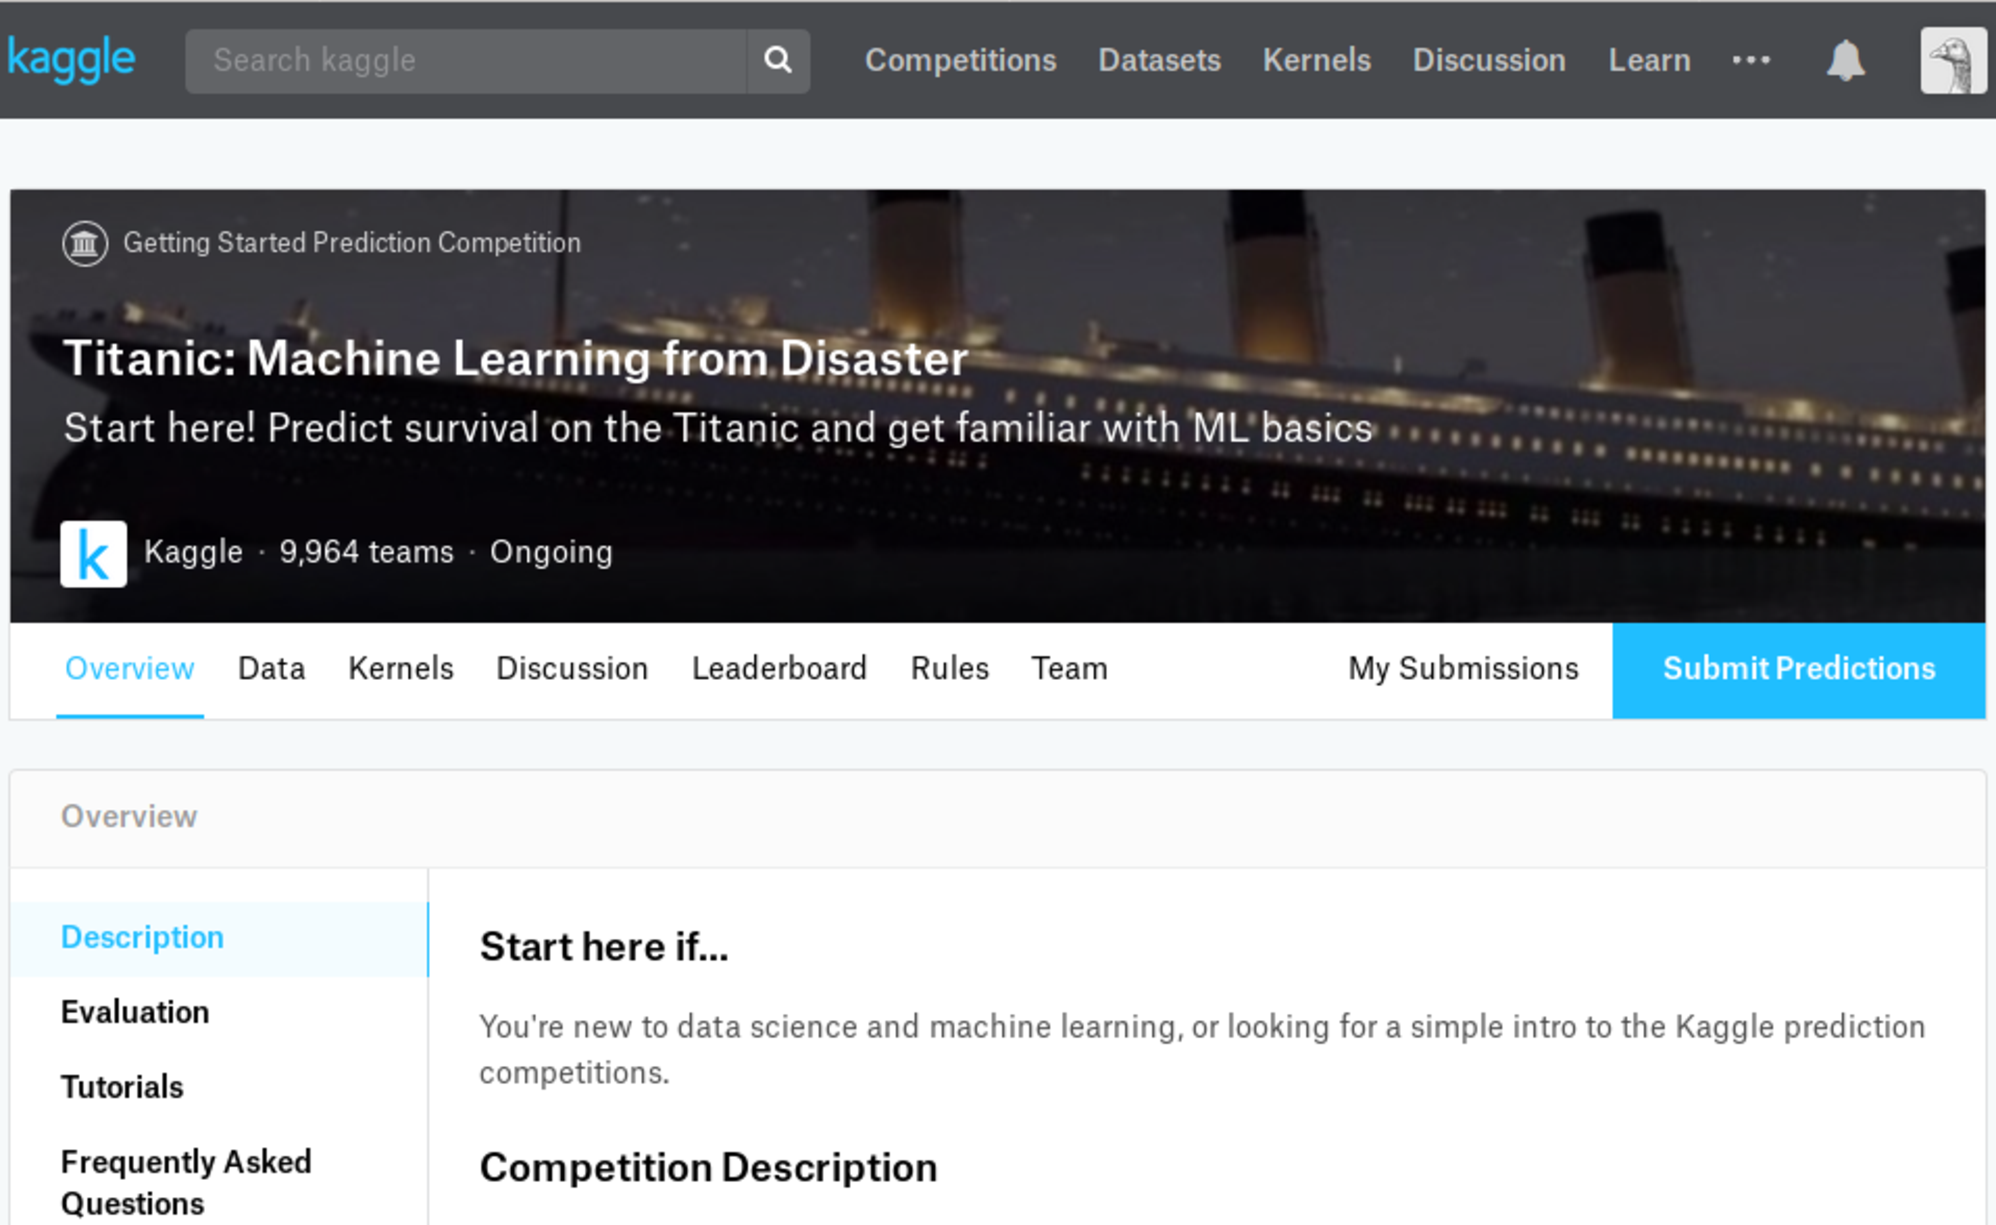
\includegraphics[width=\textwidth]{Submissao_Kaggle.pdf}
	\caption{Tela de submissão dos resultados no Kaggle.}
	\label{Fig:Submissao_KAGGLE}
\end{figure}


\chapter{Considerações Finais}

Conheça a BEMAKER nas redes sociais

\href{https://www.facebook.com/bemakerbrasil}{www.facebook.com/bemakerbrasil}

\href{https://www.instagram.com/bemakerbr}{www.instagram.com/bemakerbr}

\href{https://www.linkedin.com/company/bemakerbr/}{www.linkedin.com/company/bemakerbr/}

Bemaker - Eventos\\
Avenida Ivaí, 228, Dom Bosco\\
Belo Horizonte, MG \\

Yulab Tecnologia / Bemaker\\
Avenida Santa Matilde, 535, Dom Cabral\\
Belo Horizonte, MG \\

Este material está disponível no \href{https://gitlab.com/adelinocpp/material_didatico_workshop_machine_learning}{GitLab}.

%Links uteis

%https://www.rugged-circuits.com/10-ways-to-destroy-an-arduino


\end{document}
